\newpage
\section{线性模型}%TODO 

\subsection{引言}
\subsubsection{基本形式}
一般形式:
\begin{align*}
    f(\bm{x})=w_1x_1+w_2x_2+\dots+w_dx_d+b
\end{align*}

向量形式:
\begin{align*}
    f(\bm{x})=\bm w ^T \bm x+b
\end{align*}
其中, $\bm w=\begin{pmatrix}
    w_1 \\w_2\\ \dots \\ w_d
\end{pmatrix}, \bm x=\begin{pmatrix}
    x_1 \\x_2\\ \dots \\ x_d
\end{pmatrix}$

\subsubsection{Perceptron 感知机}
对于线性分类器, 误分类则:
\begin{align*}
    -y_i(wx_i+b)>0
\end{align*}
定义损失函数 
\begin{align*}
    L(w,b)=-\sum_{x_i\in M}y_i(wx_i+b)
\end{align*}
梯度
\begin{align*}
    \nabla_w L(w,b)&=-\sum_{x_i\in M}y_ix_i\\
    \nabla_b L(w,b)&=-\sum_{x_i\in M}y_i\\
    \therefore\ w&:=w+\eta y_ix_i\\
    b&:= b+\eta y_i
\end{align*}

\subsubsection{梯度下降}
\begin{itemize}
    \item 一阶方法
    \item 无约束优化
\end{itemize}
考虑无约束优化问题 $\displaystyle \min_{\bx} f(\bx)$, 其中 $f(\bx)$ 连续可微, 若能构造 $\bx^0, \bx^1, \bx^2,\dots$ 满足
\begin{align*}
    f(\bx^{t+1})<f(\bx^t), t=0,1,2,\dots
\end{align*}
有
\begin{align*}
    f(x+\Delta x)&=f(x)+\Delta x^\top \nabla f(x)\\
    \Delta x^\top \nabla f(x)&<0\\
    \therefore\ \Delta x&=-\gamma \nabla f(x)
\end{align*}

\subsubsection{优缺点}
优点:
\begin{itemize}
    \item 简单
    \item 可解释
    \item 基础
\end{itemize}

缺点:
\begin{itemize}
    \item 有线性不可分的数据
\end{itemize}

\subsection{回归任务}
\subsubsection{线性回归}
给定数据集 $D=\{ (\bm x_1, y_1), (\bm x_2, y_2), \dots, (\bm x_m, y_m)  \}$, 其中 $\bx_i=(x_{i1};x_{i2};\dots;x_{id})$, $y_i\in\R$. 

试图 学 得 一 个 线 性 模型 以 尽 可 能 准 确 地 预 测 实 值 输 出 标 记 .

离散属性处理:
\begin{itemize}
    \item 有序: 化为连续值
    \item 无序: 转化为 $k$ 维向量
\end{itemize}

单属性: $f(x)=wx_i+b$, 有 $f(x_i)\simeq y_i$

\paragraph{最小二乘法}
基于均方误差最小化来进行模型求解
\begin{align*}
    (w^*, b^*)&=\argmin_{(w,b)} \sum_i^m \left( f(x_i)-y_i \right)^2\\
    &=\argmin_{(w,b)} \sum_i^m \left( y_i - wx_i -b \right)^2
\end{align*}

均方误差
\begin{align*}
    E_{(w,b)}= \sum_i^m \left( y_i - wx_i -b \right)^2
\end{align*}
对 $w$ 与 $b$ 求导
\begin{align*}
    \pard{E_{(w,b)}}{w}&=\sum_i^m 2x_i\left( y_i - wx_i -b \right)\\
    &=2\left( w\sum_i^m x_i^2 -b \sum_i^m x_i + \sum_i^m x_iy_i \right)\\
    \pard{E_{(w,b)}}{b}&=\sum_i^m 2\left( y_i - wx_i -b \right)\\
    &=2\left( -w\sum_i^m x_i - mb + \sum_i^m y_i \right)
\end{align*}
令二者为0, 可得
\begin{align*}
    w&=\left( \frac{\displaystyle \sum_{i=1}^m y_ix_i- \sum_{i=1}^m y_i\sum_{i=1}^mx_i}{\displaystyle \sum_{i=1}^m x_i^2 -\frac{1}{m}\left( \sum_{i=1}^m x_i \right)^2} \right)\\
    b&=\frac{1}{m}\sum_{i=1}^m(y_i-wx_i)
\end{align*}

\subsubsection{多元线性回归}
给定数据集 $D=\{ (\bm x_1, y_1), (\bm x_2, y_2), \dots, (\bm x_m, y_m)  \}$, 其中 $\bx_i=(x_{i1};x_{i2};\dots;x_{id})$, $y_i\in\R$. 

目标: $f(\bx_i)=\bm {w}^\top \bx_i +b$, 有 $f(\bx_i)\simeq y_i$

\paragraph{齐次表达} 把 $\bm w$ 和 $b$ 吸收入向量形式 $\hat{\bm w}=(\bm w;b)$, 数据集表示为
\begin{align*}
    \bm{X}&=\begin{pmatrix}
        x_{11} & x_{12} & \cdots & x_{1d} & 1\\
        x_{21} & x_{22} & \cdots & x_{2d} & 1\\
        \vdots & \vdots & \ddots & \vdots & \vdots\\
        x_{m1} & x_{m2} & \cdots & x_{md} & 1\\
    \end{pmatrix}= \begin{pmatrix}
        \bx_1^\top & 1\\
        \bx_2^\top & 1\\
        \vdots & \vdots\\
        \bx_m^\top & 1\\
    \end{pmatrix}\\
    \by&=(y_1;y_2;\dots;y_m)
\end{align*}

\paragraph{最小二乘}类似
\begin{align*}
    \hat{\bw}^*=\argmin_{\hat{\bw}}(\by - \bm X \hat{\bw})^\top(\by - \bm X \hat{\bw})
\end{align*}
令 $E_{\hat{\bw}}= (\by - \bm X \hat{\bw})^\top(\by - \bm X \hat{\bw})$, 对 $\hat{\bw}$ 求导有
\begin{align*}
    \pard{E_{\hat{\bw}}}{\hat{\bw}}=2\bm{X}^\top(\bm{X}\hat{\bw}-\by)
\end{align*}
令其为0可得 $\hat{\bw}$ 最优解. 

\paragraph{满秩讨论}最优解涉及矩阵求逆, 比较复杂, 需要讨论. 

若 $\bm{X}^\top\bm X$ 为满秩或正定矩阵, 则
\begin{align*}
    \hat{\bw}^*=(\bm{X}^\top\bm X)^{-1}\bm{X}^\top \by
\end{align*}
线性回归模型为
\begin{align*}
    f(\hat{\bx}_i)=\hat{\bx}^\top(\bm{X}^\top\bm X)^{-1}\bm{X}^\top \by
\end{align*}

若 $\bm{X}^\top\bm X$ 不是满秩, 需要引入正则化. %TODO \ref{sec:6.4}, \ref{sec:11.4}

\subsubsection{对数线性回归}
输出标记的对数为线性模型逼近的目标
\begin{align*}
    \ln y=\bw^\top \bx +b
\end{align*}

\begin{figure}[!htb]
    \centering
    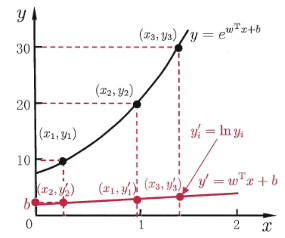
\includegraphics[width=0.309\textwidth]{pic/ML3/对数线性回归示意图}
    \caption{对数线性回归示意图}
\end{figure}


\subsubsection{广义线性模型}
考虑单调可微函数 $g(\cdot)$, 令
\begin{align*}
    y=g^{-1}\left( \bw^\top \bx+b \right)
\end{align*}
称 $g$ 为 联系函数 (link function)

\subsection{二分类任务}
%TODO 做到这里了

\subsubsection{对数几率回归}

\paragraph{对数几率函数(logistic function)}


\begin{definition}
    对数几率(log odds): 样本作为正例的相对可能性对数
    \begin{align*}
        \ln\frac{y}{1-y}
    \end{align*}
\end{definition}

优势:
\begin{enumerate}
    \item 无需假设数据分布
    \item 可得``类别''的近似概率预测
    \item 可直接应用现有数值优化算法求最优解
\end{enumerate}

\paragraph{极大似然法}


\paragraph{对数几率回归总结}
主要思想:
\begin{itemize}
    \item 引入 sigmod, 关联了离散标记与线性模型
    \item sigmod 光滑, 高阶可导, 接近离散标记
    \item 得到类别接近概率似然估计
    \item 构建极大似然目标函数
    \item 优化求解: 梯度下降, 牛顿法等
\end{itemize}


\subsubsection{线性判别分析}
(Linear Discriminant AnalysisC, LDA)
LDA 视为一种监督降维技术. 

\begin{figure}[!htb]
    \centering
    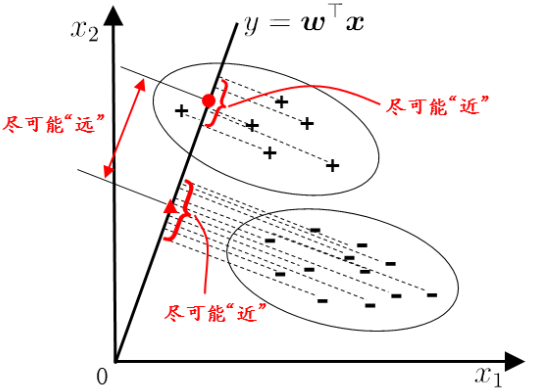
\includegraphics[width=0.309\textwidth]{pic/ML3/LDA.png}
    \caption{LDA}
\end{figure}
同类投影点尽可能接近, 异类投影点尽可能远. 

\begin{definition}\quad

    \begin{itemize}
        \item $X_i$: 第 $i$ 类示例的集合
    \end{itemize}
\end{definition}


最大化目标:
\begin{align*}
    1
\end{align*}

类内散度矩阵:
\begin{align*}
    11
\end{align*}

类间散度矩阵:
\begin{align*}
    222
\end{align*}

广义瑞利商 (generalized Rayleigh quotient)
\begin{align*}
    33
\end{align*}

令 $\bm w ^T \bm S_w \bm w=1$ 最大化上式等价形式为
\begin{align*}
    444
\end{align*}

运用拉格朗日乘子法
\begin{align*}
    555
\end{align*}

\paragraph{拉格朗日乘子法}%TODO 讲得好快()()

\paragraph{LDA推广---多分类任务}

\paragraph{LDA总结}

\subsection{多分类任务}

\subsubsection{一对一}

\subsubsection{一对其余}

\subsubsection{比较一对一与一对其余}

\subsubsection{多对多}
Many vs Many (MvM): 若干类为正类, 若干类为反类. 

\paragraph{纠错输出码} (Error Correcting Output Code, ECOC)

\begin{figure}[!htb]
    \centering
    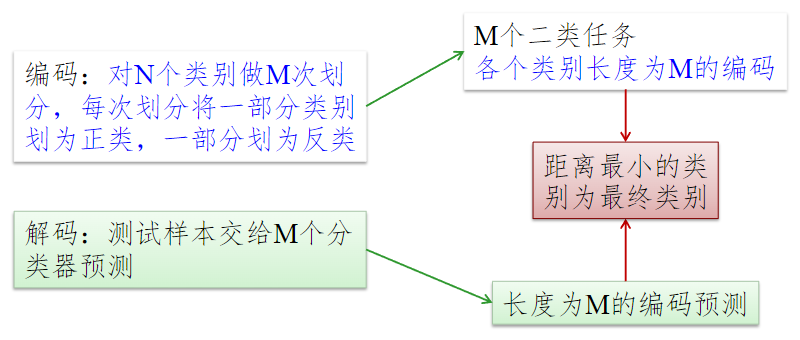
\includegraphics[width=0.42\textwidth]{pic/ML3/ECOC}
    \caption{ECOC}
\end{figure}



\subsection{类别不平衡任务}

